%!TEX root = ../../main.tex


\begin{figure}[!htb]
\centering
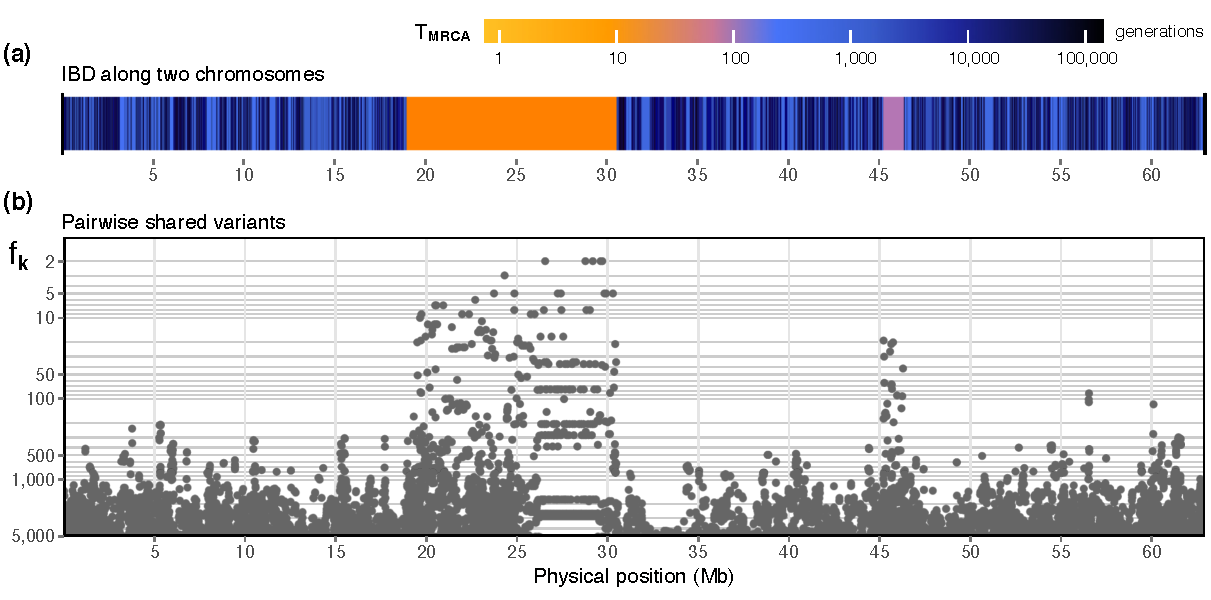
\includegraphics[width=\textwidth]{./img/ch3/pair_ibd_example}
\Caption{IBD structure and pairwise variant sharing}
{A dataset of ${N=\num{5000}}$ haplotypes was simulated under the coalescent using \texttt{msprime} \citep{Kelleher:2016fn}.
IBD status was determined from simulated genealogies for a pair of chromosomes selected at random from the set of chromosomes that shared a rare allele (frequency $\leq 0.5\%$).
Panel~\textbf{(a)} shows the ``mosaic'' of IBD segments along the full length of the simulated region for the \n{2} selected chromosomes.
The length of a given IBD segment is defined by the chromosomal interval over which the \gls{mrca} of the selected pair does not change.
The colour of each segment indicates the \gls{tmrca} for the selected pair.
Panel~\textbf{(b)} shows the physical position of \fk{} variants shared by the \n{2} chromosomes, ranging from very low allele frequency at the top (\fk{2}) to very high frequency at the bottom (\eg~\fk{>500}).
Note that the simulation was carried out under variable recombination rates using the genetic map for human chromosome~20 from the \glsentryfull{hapmap} Phase~\rom{2} Build~37.
The pattern of extended shared variation seen at positions around 25--30~\gls{Mb} arises from a low recombination rate at the region of the centromere.}
{fig:pair_ibd_example}
% \vspace{-5pt}
% \hrulefill%
\end{figure}

\glslocalresetall
